\documentclass[11pt,a4paper]{article}

\usepackage[margin=1in]{geometry}
\usepackage{hyperref}
\usepackage{enumitem}
\usepackage{graphicx}
\usepackage{xcolor}
\usepackage{float}
\usepackage{tikz}
\usetikzlibrary{shapes.geometric, arrows.meta, positioning}

% -----------------------------------------------------
% bvraghav-tiet-ucs503p-article.sty
% -----------------------------------------------------

% Variable: Lab Instructor
\makeatletter
\newcommand{\BvrSetLabInstructor}[1]{%
  \gdef\Bvr@LabInstructor{#1}}
\newcommand{\Bvr@LabInstructor}{Dr. Jeelani Asif}

% public accessor
\newcommand{\BvrLabInstructorValue}{\Bvr@LabInstructor}
\makeatother

% Add subtitle
\usepackage{titling}

% -- Set title bold
\pretitle{\begin{center}\bfseries\fontsize{18bp}{18bp}\selectfont}

\makeatletter
\newcommand{\BvrSubtitle}[1]{%
  \posttitle{%
    \par\end{center}
    \begin{center}\large#1\end{center}
    \vskip 0.5em}%
}
\makeatother

% Hints in the section title(s)
\newcommand{\BvrHint}[1]{%
  {\normalfont\normalsize\itshape\hfill #1}}

% -----------------------------------------------------

\title{AI-Enabled Smart Library Management and Resource Recommendation System}

\BvrSetLabInstructor{Dr. Jeelani Asif}

\BvrSubtitle{%
  Project Proposal for UCS503P  \\
  Submitted to: \BvrLabInstructorValue \\ \bfseries
  Thapar Institute of Engineering and Technology%
}


\author{
  Arnav Agarwal, CSED%
  \thanks{Roll No: \texttt{1024160010} \quad Email: \texttt{aagarwal_be24@thapar.edu}}
  \and
  Aradhya Goyal, CSED%
  \thanks{Roll No: \texttt{1024160135} \quad Email: \texttt{agoyal15_be24@thapar.edu}}
  \and
  Amanjot Kaur Sidhu, CSED%
  \thanks{Roll No: \texttt{1024160025} \quad Email: \texttt{asidhu1_be24@thapar.edu}}
}

\date{29 August, 2026}

\begin{document}

\maketitle

\begin{abstract}
University libraries manage large collections of books and other learning resources while handling student records, issue and return transactions, overdue items, fines, and resource availability. Conventional library management systems primarily provide storage, search, and CRUD-based operations, leaving several administrative activities manual and reactive. This project proposes a web-based Smart Library Management System that combines conventional library workflows with a lightweight multi-agent artificial intelligence layer. The proposed system consists of three specialized agents: a Library Intelligence Agent for natural-language resource discovery and recommendation, a Record Onboarding Agent for validating and importing student records, and a Library Monitoring Agent for overdue monitoring, notifications, and resource-demand analysis. The system integrates these agents with application APIs and a MySQL database so that AI-assisted operations are grounded in actual library data. The project emphasizes rapid incremental delivery, CI/CD, measurable evaluation, and practical deployment rather than novel AI research.
\end{abstract}

\section{Higher-Order Goal}
The higher-order goal of this project is to improve the efficiency and accessibility of university library services through software automation and data-driven resource management. The immediate engineering objective is to reduce the time and effort involved in common library workflows while providing students and administrators with a unified and deployable software platform.

The project uses artificial intelligence as an enabling technology rather than as a research objective. The primary focus remains on dependable software engineering, workflow automation, system integration, and measurable improvement in library operations.

\section{Time-to-Value}
The project is designed around rapid delivery and short feedback cycles.
\begin{itemize}
    \item A usable minimum viable product (MVP) will be implemented during the initial iteration, including authentication, resource management, resource search, issue/return workflows, and database integration.
    \item AI-assisted functionality will be introduced incrementally after the core library workflow is operational.
    \item CI will be established early so that every code change is automatically checked through linting, testing, and build validation.
    \item Subsequent iterations will add AI-assisted resource discovery, record onboarding, monitoring, and resource-demand analysis.
    \item Each iteration will produce a demonstrable increment that can be tested independently and improved using feedback.
\end{itemize}
The project therefore prioritizes fast feedback over attempting to implement the complete feature set at the beginning of the semester.

\section{Problem Statement}
University libraries handle a large number of resource records, student records, borrowing transactions, and overdue items. Although conventional library systems can store and retrieve these records, several operational problems remain.
\begin{itemize}
    \item \textbf{Manual resource discovery:} Students may need to navigate through multiple search and filtering options to determine whether a suitable resource is available.
    \item \textbf{Manual record onboarding:} Importing large numbers of student or member records can require repetitive validation and manual duplicate checking.
    \item \textbf{Reactive overdue management:} Overdue resources are often identified only after staff manually inspect issue and due-date records.
    \item \textbf{Limited demand visibility:} Library administrators may not have an immediate way to identify frequently issued resources with insufficient available copies.
    \item \textbf{Data without assistance:} A conventional database stores library information but does not directly assist users in converting that information into actionable answers or recommendations.
\end{itemize}
\textbf{Why this matters now (contextual relevance):} A university library serves a large student population with continuously changing resource requirements. Improving resource discovery, record processing, overdue monitoring, and demand visibility can reduce repetitive administrative effort and improve the usability of existing library resources.

\section{Proposed Solution}
\subsection{Overview}
We propose a web-based Smart Library Management System consisting of a student interface, an administrator interface, application APIs, a MySQL database, and a controlled AI agent layer.

The system will provide the following core capabilities:
\begin{itemize}
    \item \textbf{Resource management:} maintain records of books and other library-managed resources, including availability and issue status.
    \item \textbf{Student/member management:} create, update, search, and import student records.
    \item \textbf{Issue and return workflow:} record borrowing transactions, due dates, returns, and applicable fines.
    \item \textbf{Natural-language resource discovery:} allow students to search for suitable resources using ordinary language.
    \item \textbf{Automated monitoring:} detect overdue resources and initiate notification and fine-related workflows.
    \item \textbf{Demand analysis:} identify heavily issued resources with limited availability and generate purchase recommendations for administrators.
\end{itemize}

\subsection{Core Workflow}
The core workflow is divided into conventional software functionality and AI-assisted functionality.
\begin{enumerate}
    \item A student authenticates and searches or requests a library resource.
    \item The backend retrieves resource records and availability from the MySQL database.
    \item For natural-language requests, the Library Intelligence Agent interprets the request and retrieves relevant information through controlled application tools.
    \item The student issues an available resource, and the backend records the transaction and due date.
    \item The Library Monitoring Agent periodically checks borrowing records and identifies resources approaching or exceeding their due dates.
    \item The system generates reminders and updates relevant workflow records.
    \item Historical issue data is analyzed to identify high-demand resources with comparatively low availability.
    \item The administrator receives demand-based recommendations for acquiring additional copies or improving resource allocation.
\end{enumerate}

\subsection{Operational Constraints}
\begin{itemize}
    \item The system will use responsive web interfaces so that it remains usable on common student and administrative devices.
    \item AI functionality will rely on mature software libraries and available APIs rather than requiring novel model training.
    \item AI agents will operate through controlled application APIs or tools rather than unrestricted direct database access.
    \item Conventional database queries will be used whenever deterministic logic is sufficient; AI will be used where natural-language interaction, recommendation, summarization, or pattern interpretation provides additional value.
\end{itemize}

\section{Solution Approach}
This project is an engineering-focused software system. The implementation will emphasize modular design, reliable workflows, automated testing, deployment, and measurement rather than novel AI algorithm research.

\subsection{Web Architecture}
The proposed system follows a modular 3-tier web architecture integrated with a controlled AI agent layer:

\begin{figure}[H]
\centering
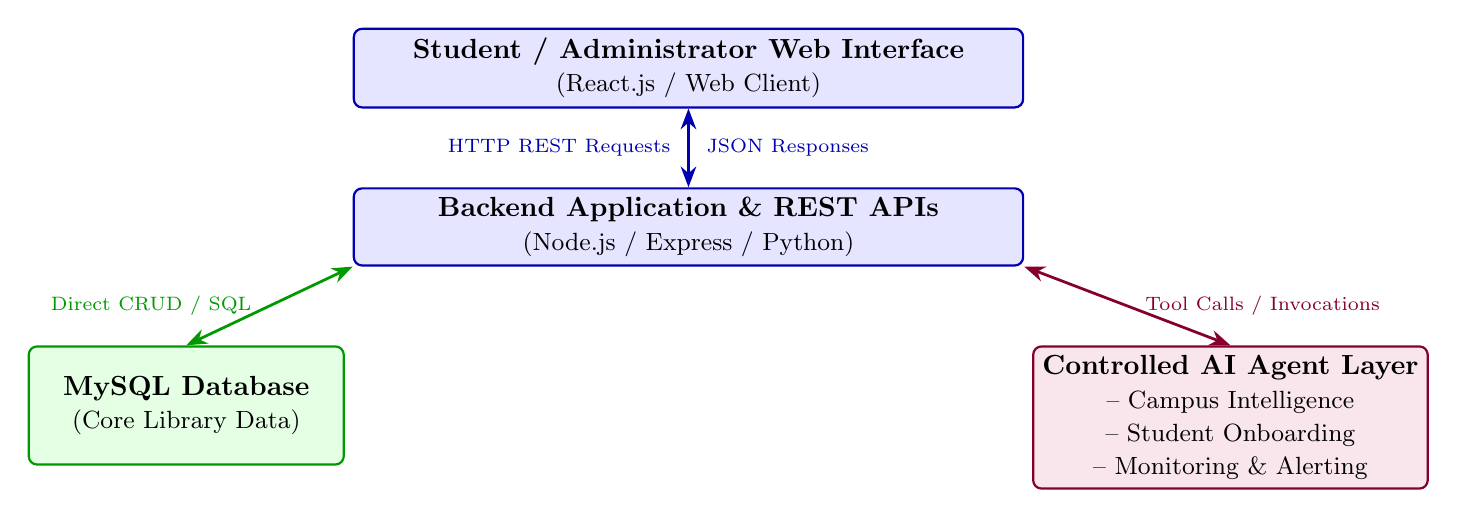
\begin{tikzpicture}[
    box/.style={rectangle, draw=blue!70!black, fill=blue!10, thick, minimum width=8.5cm, minimum height=0.9cm, align=center, rounded corners=3pt},
    midbox/.style={rectangle, draw=blue!70!black, fill=blue!10, thick, minimum width=8.5cm, minimum height=0.9cm, align=center, rounded corners=3pt},
    smallbox/.style={rectangle, draw=green!60!black, fill=green!10, thick, minimum width=4cm, minimum height=1.5cm, align=center, rounded corners=3pt},
    aibox/.style={rectangle, draw=purple!70!black, fill=purple!10, thick, minimum width=4cm, minimum height=1.5cm, align=center, rounded corners=3pt},
    arrow/.style={<->, >=Stealth, thick, line width=1pt}
]

\node (fe) [box] {\textbf{Student / Administrator Web Interface}\\ \small(React.js / Web Client)};
\node (be) [midbox, below=1cm of fe] {\textbf{Backend Application \& REST APIs}\\ \small(Node.js / Express / Python)};
\node (db) [smallbox, below left=1cm and 0.1cm of be] {\textbf{MySQL Database}\\ \small(Core Library Data)};
\node (ai) [aibox, below right=1cm and 0.1cm of be] {\textbf{Controlled AI Agent Layer}\\ \small-- Campus Intelligence\\ \small-- Student Onboarding\\ \small-- Monitoring \& Alerting};

\draw [arrow, color=blue!70!black] (fe) -- node[left, font=\scriptsize, align=right] {HTTP REST Requests\ } node[right, font=\scriptsize, align=left] {\ JSON Responses} (be);
\draw [arrow, color=green!60!black] (be.south west) -- node[left, font=\scriptsize, align=right] {Direct CRUD / SQL\ } (db.north);
\draw [arrow, color=purple!70!black] (be.south east) -- node[right, font=\scriptsize, align=left] {\ Tool Calls / Invocations} (ai.north);

\end{tikzpicture}
\caption{Modular 3-Tier Web Architecture with Integrated AI Agent Layer.}
\label{fig:web_architecture}
\end{figure}

\subsection{System Design and Data Flow Diagrams}

\subsubsection{Use Case Diagram}
Figure~\ref{fig:use_case} defines the interactions between human actors (\textit{Students}, \textit{Librarian}) and system agents (\textit{Monitoring and Notification Agent}, \textit{Student Onboarding Agent}, \textit{Campus Intelligence Agent}).

\begin{figure}[H]
    \centering
    \fbox{
\includegraphics[width=0.75\textwidth,height=0.4\textheight,keepaspectratio]{Use-Case-Diagram.png}}
    \caption{Use Case Diagram showing human actor and AI agent interactions.}
    \label{fig:use_case}
\end{figure}

\subsubsection{Data Flow Diagram (Level 0 - Context Diagram)}
The Level 0 Context Diagram (Figure~\ref{fig:dfd_level0}) illustrates the system boundary, mapping global data exchanges between external actors, AI agents, and the primary system process.

\begin{figure}[H]
    \centering
    \fbox{
\includegraphics[width=0.8\textwidth,height=0.4\textheight,keepaspectratio]{Level_0_DFD.png}}
    \caption{Level 0 Context Data Flow Diagram (DFD).}
    \label{fig:dfd_level0}
\end{figure}

\subsubsection{Data Flow Diagram (Level 1 - System Subsystems)}
Figure~\ref{fig:dfd_level1} decomposes the system into core functional processes (\textit{1.0 Search and Intelligent Assistance}, \textit{2.0 Records \& Asset Management}, \textit{3.0 Circulation and Fine Tracking}, \textit{4.0 Monitoring and Alert Generation}) and links them to primary data stores.

\begin{figure}[H]
    \centering
    \fbox{\includegraphics[width=0.75\textwidth,height=0.45\textheight,keepaspectratio]{Level_1_DFD.png}}
    \caption{Level 1 Data Flow Diagram (DFD) showing internal subsystems and data stores.}
    \label{fig:dfd_level1}
\end{figure}

\subsubsection{Data Flow Diagram (Level 2 - Process 1.0 Breakdown)}
Figure~\ref{fig:dfd_level2} details the internal operations of Process 1.0 (\textit{Search and Intelligent Assistance}), showing query parsing (1.1), catalog querying (1.2), and context recommendation generation (1.3) in coordination with the Campus Intelligence Agent.

\begin{figure}[H]
    \centering
    \fbox{
\includegraphics[width=0.75\textwidth,height=0.4\textheight,keepaspectratio]{Level_2_DFD.png}}
    \caption{Level 2 Data Flow Diagram (DFD) for Intelligent Search (Process 1.0).}
    \label{fig:dfd_level2}
\end{figure}

\subsection{Library Intelligence Agent}
The Library Intelligence Agent is intended for students and administrators. Its responsibilities include:
\begin{itemize}
    \item interpreting natural-language resource requests,
    \item searching library resources through application APIs,
    \item providing availability-aware recommendations,
    \item answering common resource-related queries, and
    \item generating concise summaries from library data where appropriate.
\end{itemize}

\subsection{Record Onboarding Agent}
The Record Onboarding Agent assists administrators with bulk student or member imports. Its responsibilities include:
\begin{itemize}
    \item uploading structured records,
    \item validating required fields,
    \item detecting likely duplicate records,
    \item inserting valid records through controlled backend operations, and
    \item generating an import summary for the administrator.
\end{itemize}

\subsection{Library Monitoring Agent}
The Library Monitoring Agent is responsible for scheduled monitoring and resource-management assistance. Its responsibilities include:
\begin{itemize}
    \item detecting resources approaching their due date,
    \item detecting overdue resources,
    \item initiating reminder and fine-related workflows,
    \item analyzing issue frequency and resource availability, and
    \item identifying high-demand resources for purchase consideration.
\end{itemize}

\subsection{AI Safety and Control}
AI-assisted operations will be constrained by the backend application. Agents will not receive unrestricted SQL access, and database modifications will occur through predefined application APIs or tools.

\subsection{CI/CD and Fast Delivery}
CI/CD will support frequent and repeatable releases. The CI pipeline will install dependencies, execute linting and static checks, run automated tests, and deploy successful builds to staging/production environments.

\section{Evaluation Criterion}
The success of the project will be evaluated using measurable metrics related to the main workflows.

\subsection{Primary Evaluation Metrics}
\begin{itemize}
    \item \textbf{Resource discovery time:} median time required for a user to locate a requested or suitable available resource. Target: less than or equal to 10 seconds for predefined test queries.
    \item \textbf{Duplicate detection precision:} proportion of records flagged as duplicates that are actually duplicates in a labeled test dataset. Target: at least 90\%.
    \item \textbf{Overdue detection coverage:} proportion of overdue transactions correctly identified by the monitoring workflow. Target: at least 99\% during controlled testing.
    \item \textbf{Demand recommendation accuracy:} proportion of high-demand/low-availability resources correctly identified according to predefined thresholds. Target: at least 90\%.
\end{itemize}

\subsection{Secondary Evaluation Metrics}
\begin{itemize}
    \item \textbf{API response time:} median response time for common non-AI application requests. Target: less than or equal to 500 ms under normal test load.
    \item \textbf{AI answer validity:} proportion of predefined library questions for which the agent returns information consistent with the database. Target: at least 90\%.
    \item \textbf{Notification delay:} time between an overdue condition becoming eligible and generation of the corresponding notification.
    \item \textbf{System reliability:} availability of the deployed application during the pilot period. Target: at least 99\%.
    \item \textbf{Test coverage:} percentage of critical backend logic covered by automated tests. Target: at least 70\%.
\end{itemize}

\subsection{Baseline and Validation Plan}
Evaluation will use controlled datasets and predefined test scenarios.
For resource discovery, the team will measure the time required to locate resources using the conventional interface and compare it with the natural-language interaction.
For onboarding, a labeled dataset containing valid, invalid, and duplicate records will be created to measure processing time and duplicate-detection precision.
For monitoring, synthetic borrowing records with known due dates and overdue states will be used to measure detection coverage and notification latency.
For demand analysis, historical or synthetic issue records will be used to define high-demand resources using predetermined thresholds. The resulting recommendations will then be compared against the expected labels.

\section{Scalability}
The system is designed to scale in both theoretical and practical terms.

\subsection{Logical Scalability}
\begin{itemize}
    \item Frontend and backend responsibilities are separated.
    \item Backend APIs are designed to be stateless where practical.
    \item Database queries will use indexing and pagination for frequently accessed records.
    \item AI agents are modular and can be extended or replaced without rewriting the complete application.
\end{itemize}

\subsection{Operational Deployability}
\begin{itemize}
    \item The application can be containerized using Docker.
    \item A managed relational database can be used for deployment.
    \item CI/CD supports repeatable staging and production deployments.
    \item The architecture can support a larger number of users and records without requiring a fundamental redesign.
\end{itemize}

\section{Engine Availability Heuristic}
The project relies on mature and readily available software engines rather than requiring fundamental algorithmic research.
\begin{itemize}
    \item A modern web framework for frontend and backend development.
    \item REST API infrastructure for application integration.
    \item MySQL or another managed relational database.
    \item Authentication and role-based authorization libraries.
    \item Mature LLM or AI APIs and supporting agent frameworks.
    \item Automated testing frameworks for unit and integration testing.
    \item GitHub Actions or an equivalent CI runner.
    \item Docker and a platform-hosted or cloud deployment target.
\end{itemize}

\section{Project Scope and Deliverables}
\subsection{Initial MVP}
\begin{itemize}
    \item Student and administrator authentication.
    \item Role-based access control.
    \item Library resource and student record management.
    \item Resource search and availability display.
    \item Issue and return workflow.
    \item Basic due-date and fine tracking.
    \item MySQL database integration.
    \item Backend API and frontend integration.
    \item CI pipeline with automated tests and linting.
\end{itemize}

\subsection{Subsequent Deliverables}
\begin{itemize}
    \item Natural-language resource discovery.
    \item AI-based resource recommendation.
    \item Bulk student/member onboarding with duplicate detection.
    \item Automated overdue monitoring and notifications.
    \item Demand analysis for frequently issued and low-availability resources.
    \item Purchase recommendations for library administrators.
    \item Administrative analytics and reporting.
    \item Search, filtering, and database performance improvements.
\end{itemize}

\subsection{Final Prototype}
The final prototype will integrate the major modules into a deployable system and demonstrate end-to-end student and administrator workflows, all three AI-assisted modules, automated testing and CI/CD, measurable evaluation results, scalability-oriented implementation decisions, and deployment on an accessible hosting environment.

\section{Timeline}
\begin{table}[H]
\centering
\begin{tabular}{|l|p{5cm}|p{7cm}|}
\hline
\textbf{Week} & \textbf{Primary Task} & \textbf{Expected Deliverable} \\ \hline
W1 & Project setup and Requirements & Requirements, repository, initial architecture \\ \hline
W2 & Database and backend foundation & Database schema, APIs, CI pipeline \\ \hline
W3 & Authentication and core library workflows & Login, roles, resource and student modules \\ \hline
W4 & Proposal completion and MVP integration & Initial integrated MVP \\ \hline
W5 & Search, issue, return, and fine workflows & Functional library transaction system \\ \hline
W6 & Testing and deployment & Automated tests and staging deployment \\ \hline
W7 & First prototype & Working MVP demonstration \\ \hline
W8 & Feedback and improvement plan & Measured feedback and prioritized improvements \\ \hline
W9 & Library Intelligence Agent & Natural-language resource discovery \\ \hline
W10 & Recommendation functionality & Availability-aware resource recommendations \\ \hline
W11 & Record Onboarding Agent & Bulk import and duplicate detection \\ \hline
W12 & Library Monitoring Agent & Overdue detection and notification workflow \\ \hline
W13 & Demand analysis & High-demand/low-availability detection \\ \hline
W14 & Integration and performance testing & Integrated second-stage system \\ \hline
W15 & Second prototype & Second prototype demonstration \\ \hline
W16 & Refinement and final testing & Bug fixes, optimization, final evaluation \\ \hline
W17 & Final prototype and presentation & Final deployed system, report, and presentation \\ \hline
\end{tabular}
\end{table}

\section{Risks and Mitigations}
\begin{itemize}
    \item \textbf{AI hallucination or incorrect resource information:} AI responses will be grounded in current database records through controlled retrieval tools and predefined APIs.
    \item \textbf{Excessive project scope:} The core library workflow will be completed before AI features are added, and later functionality will be delivered incrementally.
    \item \textbf{Duplicate detection errors:} Potential duplicates will be flagged for human review instead of being automatically deleted.
    \item \textbf{AI service unavailability:} Conventional keyword-based resource search will remain available as a fallback.
    \item \textbf{Unauthorized automated actions:} Agents will operate through role-controlled APIs, and irreversible operations will require explicit backend authorization.
    \item \textbf{Insufficient evaluation data:} Synthetic and labeled library datasets will be prepared early so that evaluation does not depend entirely on access to live institutional data.
    \item \textbf{Deployment instability:} A staging environment and CI/CD pipeline will be established early to make deployments repeatable.
    \item \textbf{Database performance degradation:} Frequently accessed fields will be indexed and database operations will use pagination and optimized queries.
\end{itemize}

\section{Summary}
This project proposes a deployable AI-enabled Smart Library Management System that combines conventional library workflows with carefully scoped AI-assisted functionality. The system addresses practical problems in resource discovery, record onboarding, overdue monitoring, and resource demand analysis.

The project aligns with software engineering requirements by prioritizing rapid time-to-value, incremental delivery, CI/CD, mature engineering engines, scalability, and measurable evaluation. A working MVP will be produced early and subsequently extended through AI-assisted resource discovery, onboarding, monitoring, and demand-based recommendations.

The system will be evaluated using measurable workflow, accuracy, performance, and reliability metrics rather than relying only on qualitative claims. The project therefore focuses on building and validating a practical, scalable, and deployable library-management platform rather than pursuing novel AI research.

\end{document}
